	Acerca do projeto da bancada de testes não destrutivos para amortecedores de carros populares,descreve-se a seguir as definições de projeto da área de eletrônica.

	\textbf{Objetivo}

	Desenvolver a central de controle da bancada e sensoreamento de parâmetros do projeto.

	\textbf{EAP}

	Na EAP do projeto eletrônico, mostrada na Figura \ref{EAPeletronica}, apresenta-se o detalhamento dos pacotes de trabalho e os entregáveis definidos para o desenvolvimento do projeto eletrônico.

	\begin{figure}[!h]
		\centering
		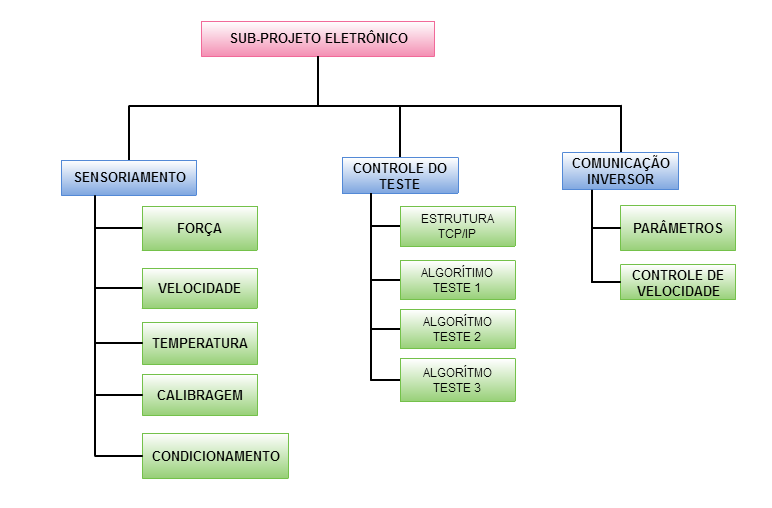
\includegraphics[scale=0.6]{EAPeletronica.png}
		\caption{Estrutura Analítica do Projeto Eletrônico}
		\label{EAPeletronica}
	\end{figure}


	Nos parágrafos a seguir descreve-se brevemente os pacotes de trabalho apresentados na EAP do projeto eletrônico. 

	\textit{Sensoriamento}: Corresponde ao sistema responsável por realizar a aquisição dos dados referente à temperatura do amortecedor, à força de reação do amortecedor e a velocidade da haste. O desenvolvimento de rotinas de calibração e a construção do circuito de condicionamento desses sinais também estão compreendidos nesse pacote de trabalho.

	\textit{Controle do Teste}: Esse ramo da EAP corresponde ao desenvolvimento dos algorítmos de controle de execução dos testes a partir dos dados recebidos, através de protocolo TCP/IP, informados pelo usuário. 

	\textit{Comunicação com o inversor}: Esse ramo compreende ao interfaceamento entre a sída da BBB e a entrada analógica do inversor, logo aspectos como a parametrização e a configuração do inversor também estão incluídos.

	\textbf{Lista É / Não É}

	\textit{ É função da equipe do projeto eletrônico:}

	\begin{itemize}

	\item Selecionar os sensores, dada as especificações exigidas pelo projeto, que devem ser obtidas dos subgrupos da área de Mecânica e Elétrica.
	\item Interfacear os sensores com a central, usando a plataforma da própria BBB.
	\item Desenvolver o sistema de comunicação da central usando um sistema linux. A central deverá estabelecer a comunicação (servidor e cliente) usando o protocolo TCP/IP.
	\item Controlar o motor AC trifásico, interfaceando o inversor com a BBB.
	\item Salvar os resultados em uma EEPROM.
	\item Prototipar uma placa de circuito impresso para o interfaceamento físico entre os sensores e a BBB.
	\item Desenvolver algorítmo de controle de execução do teste.

	\end{itemize}

	\textit{ Não é função da equipe do projeto eletrônico:}

	\begin{itemize}

	\item Desenvolver o sistema elétrico de acionamento da bancada.
	\item Desenvolver a fonte de conversão de 220AC para 5V DC.
	\item Desenvolver a interface gráfica para acionamento remoto (usando o cliente) da bancada.
	\item Definir quaisquer variáveis acerca do projeto mecânico, amortecedor e temperatura.

	\end{itemize}

	\textbf{Requisitos}

	Dada as definições de testes que serão executados na bancada, o sistema eletrônico deverá ser capaz de obter os parâmetros exigidos, tais como temperatura do amortecedor, velocidade linear da haste e força de reação do amortecedor; além disso, o sistema deverá ser desenvolvido com o protocolo TCP/IP, para permitir que seja desenvolvida a interface gráfica que irá controlar a bancada remotamente. O resultado deverá ser salvo em um sistema não volátil, para assegurar que caso ocorra alguma falha energética, os mesmos não se percam. Os sensores devem ser dimensionados de modo a satisfazer as condições de operação do teste. 

	\textbf{Propósito}

	Para a realização dos testes no amortecedor, existe a necessidade de obter parâmetros para a validação da especificação teórica, no que se refere a funcionalidade do amortecedor. Com isso, é necessário o desenvolvimento de um sistema que controle tanto as obtenções dos parâmetros exigidos, quanto o controle do teste e armazenamento dos resultados.

	\textbf{Stakeholders}

	Os integrantes Eduardo e Regina compõem a equipe de desenvolvimento eletrônico e estão diretamente relacionados. As equipes do desenvolvimento da aplicação web, formada pelos estudantes de engenharia de software, e a equipe de especificação e controle do motor, formada pelos estudantes de engenharia de energia, também estão envolvidos no projeto por haver pontos importantes de interação no processo de desenvolvimento.

	\textbf{Espectativa dos Stakeholders}

	Segundo a Figura \ref{EAPeletronica} mostra, tem-se a expectativa de entregar para o segundo ponto de controle a PCI de condicionamento, estrutura preliminar do algorítimo de controle dos testes, estrutura TCP/IP, algorítmo de aquisição dos dados de força, algorítmo de aquisição dos dados de proximidade.
	Para o terceiro ponto de controle espera-se entregaro sistema de controle de testes, os algorítmos de aquisição dos dados de temperatura, parametrização do inversor e implementação das rotinas de calibragem.

	\textbf{Premissas}

	Para a execução do projeto eletrônico da bancada, considera-se verdadeiro as seguintes situações:
	\begin{itemize}

	\item As definições mecânicas estão bem definidas e não sofrerão alterações. O conjunto de sensores irão, além de captar dados importantes para as conclusões do teste do amortecedor, ser responsáveis pelo funcionamento da bancada. O dispositivo eletrônico, em nível de programação, ou seja, o controle da bancada por meio do sistema cliente/servidor, dado as informações capturadas pelos sensores requer a funcionalidade bem definida.
	\item O inversor de frequência, usado para controlar o motor elétrico, é compatível com o hardware (placa beaglebone). Isso permitirá o pleno controle por meio do sistema operacional embarcado.
	Dada as especificações de quais parâmetros devem ser adquiridos, os sensores necessários para tal tarefa devem estar disponíveis dentro do prazo definido para a etapa de instanciar os sensores no hardware e software escolhidos.
	\item O sistema embarcado deve atender a necessidade do projeto. Isso significa que todos os dados dos sensores devem obtidos, gravados e transmitidos para o cliente, que em nível de protótipo (no terminal) deve ser desenvolvido pela equipe de eletrônica e em nível de produto final será desenvolvido pela equipe de software.
	\item As definições elétricas, ou seja, alimentação do sistema eletrônico e de toda a bancada, devem ser desenvolvidos. Os circuitos necessários e placas de circuito impresso devem ser projetadas, testadas e instaladas no projeto.

	\end{itemize}

	\textbf{Restrições Organizacionais}

	Em virtude da divisão do grupo em equipes de desenvolvimento em função da sua áreas de formação e atuação no projeto, assim como a quantidade de integrantes que cursam engenharia eletrônica, o presente projeto possui pouca versatilidade para a equipe do projeto eletrônico, logo a equipe de desenvolvimento do projeto eletrônico não foi subdividida.

	\textbf{Investimento}

	A tabela \ref{investimentoeletronica} apresenta uma descrição do investimento do projeto para aquisição de componentes eletrônicos.

	\begin{table}[!h]
	\centering
	\caption{Investimento do Projeto Eletrônico}
	\vspace{0.5cm}
	\begin{tabular}{ c c}
	\hline
	\textbf{DESCRIÇÃO}	&	\textbf{VALOR (R\$)}\\
	\hline
	Célula de Carga & 506,26 \\
	\hline
	MLX90614 & 155,00\\
	\hline
	BBB & 0,00\\
	\hline
	HC-SR04 & 0,00\\
	\hline
	Componentes Diversos & 30,00\\
	\hline
	\textbf{TOTAL} & \textbf{691,26}\\
	\hline

	\label{investimentoeletronica}
	\end{tabular}
	\end{table}

	\textbf{Riscos}

	Acerca do sistema eletrônico, tem-se os seguintes riscos:
	\begin{itemize}

	\item Quebra de um dos sensores: Isso resultará em atrasos, dado que os sensores foram comprados de outra cidade e tem-se o prazo de entrega envolvido no processo de aquisição. Além disso, os custos do projeto aumentarão.
	\item Dificuldade na implementação do servidor junto aos sensores: Isso resultará no mínimo em atrasos e em um caso extremo, na inviabilidade do projeto. Para contornar esse problema, os módulos já estão sendo construídos e testados isoladamente.
	\item Dificuldade na instanciação do inversor de frequência: O inversor foi construído para operar com o uso de uma CLP, sendo assim, há a necessidade de entender o protocolo de comunicação do sistema original, para então recriá-lo no nosso sistema. Essa dificuldade é proporcional a nossa disponibilidade com o uso do equipamento, dado que ele é de propriedade da universidade.
	\item Necessidade de adicionar ou substituir sensores devido a novas especificações de projeto: Isso pode resultar em atrasos, perca parcial ou completa de implementações já realizadas.

	\end{itemize}

	\textbf{Descrição dos subprodutos identificados}

	\begin{itemize}

	\item PCI de condicionamento: Refere-se a prototipação de uma PCI que contém os bornes para conexão dos sensores e do inversor com a BBB, bem como os circuitos de condicionamento para cada sensor.
	\item Estrutura TCP/IP: Trata-se da construção da arquitetura de comunicação entre o cliente e o servidor para tráfego das informações do usuário e os resultados do teste.
	\item Algorítmo de aquisição dos dados de temperatura: Corresponde ao código em que é realizado o recebimento dos sinais digitais provenientes do MLX90614 e a conversão dos mesmos em termos de temperatura em graus Celsius , por ultimo os dados do teste são armazenados em um arquivo em formato txt.
	\item Algorítmo de aquisição dos dados de força: Corresponde ao código em que é implementado um conversor A/D, um conversor de dados digitais para informações em termos de força a partir da curva de sensibilidade do sensor e por ultimo os dados do teste são armazenados em um arquivo em formato txt.
	\item Algorítmo de aquisição dos dados de velocidade: Corresponde ao código em que é realizado a aferição do tempo em que o pino ECHO permanece em nível lógico para aferição da distância do objeto assim como uma função que realiza o cálculo da taxa de variação dessa posição no tempo de amostragem para obtenção da velocidade linear da haste, por ultimo os dados do teste são armazenados em um arquivo em formato txt.
	\item Algorítmo de controle de teste: Corresponde ao módulo que recebe os dados provenientes da aplicação web e aciona a saída PWM em função das características do teste inseridas pelo usuário.
	\item Interfaceamento BBB com o inversor: Corresponde ao módulo de amplificação do sinal de saída da BBB para inserção na entrada analógica do inversor para controle de velocidade.
	\end{itemize}

\newpage
\subsection{Proposta Eletrônica}

	A Figura \ref{sistema} exemplifica de maneira bastante simplificada o sistema proposto.

	\begin{figure}[!h]
		\centering
		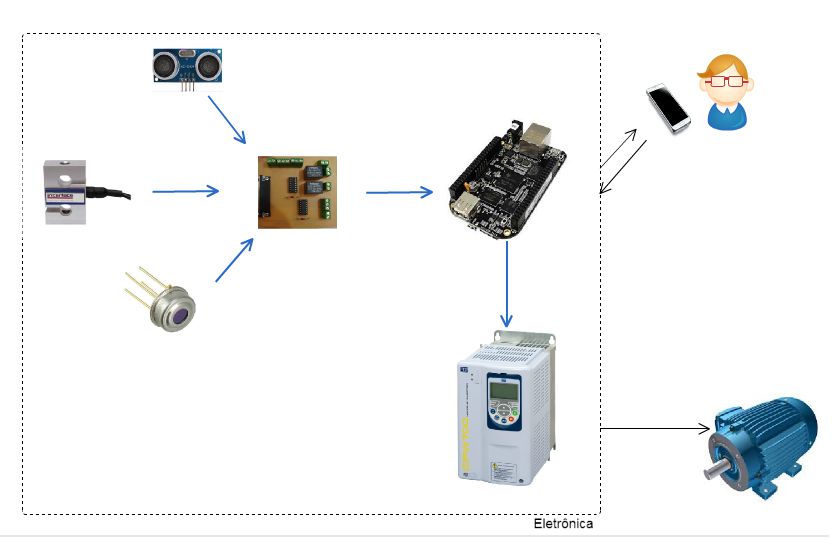
\includegraphics[scale=0.5]{sistema.png}
		\caption{Sistema proposto simplificado}
		\label{sistema}
	\end{figure}

	Em linhas gerais,a bancada, em termos de componentes eletrôncos, está equipada com:

	\begin{itemize}

	\item Kit BeagleBone, placa e módulo de conexão wi-fi, onde será embarcado o software de recebimento, processamento e interfaceamento dos dados;
	\item Sensor HC-SR04, reponsável por realizar a aferição da distãncia entre a base da haste do amortecedor e a base da bancada, a ser utilizado posteriormente como medição indireta de velocidade;
	\item Sensor MLX90614, responsável por realizar a medição da temperatura do amortecedor através de infravermelho;
	\item Célula de Carga IWM ZSL 500kg, disposisitivo utilizado na medição da força de reação do amortecedor ao movimento de excitação;
	\item PCI de circuito condicionador de sinal, circuito desenvolvido com o objetivo de preparar os sinais provenientes dos sensores para conexão com os pinos da BBB;
	\item Inversor de Frequência WEG CFW11.10 responsável por realizar o controle da rotação do motor em detrimento dos sinais analógicos provenientes da BBB;
	\item Uma fonte Minipa.
	\end{itemize}	

\subsection{Descrição da solução}
	
	Descreve-se nessa seção os circuitos implementados para aquisição dos dados dos sensores e interfaceamento com a Beaglebone.

	\subsubsection{Escolha do hardware: \emph{Beaglebone Black}}
	A \emph{Beaglebone Black} é uma placa que possui um hardware completo para aplicações industriais. Possui um processador ARM Cortex A8, 512MB de memória RAM, 4GB de armazenamento flash, noventa e dois pinos, dos quais sessenta e cinco são \emph{GPIO}, com sete entradas analógicas e duas PRU - \emph{Programmable Realtime Unit Subsystem}. Essa configuração permite o uso de um sistema operacional embarcado com instruções em linguagens de programação de alto nível, comparadas com as instruções normalmente usadas em microcontroladores. Como o projeto tem como base a instanciação de uma rede de sensores, o fato da placa possuir entrada analógica é um dos pontos decisivos na escolha da \emph{Beaglebone Black}.

	Caso fosse escolhida uma outra plataforma, como a \emph{Raspberry Pi}, teríamos custos adicionais no projeto, com a compra de conversores analógico/digital ou um microcontrolador para instanciar a rede de sensores. O caso mais crítico observado seria com o uso de um microcontrolador adicional, resultando na implementação de uma Raspberry Pi recebendo via serial os dados dos sensores instanciados em um Arduino ou placas semelhantes. Tal abordagem acarreta em um desperdício de hardware e iria contra o intuito da disciplina, que é aproximar os estudantes do desenvolvimento de projeto a nível industrial, ou seja, menor custo com a melhor eficiência possível.

	Usando a \emph{Beaglebone Black}, traçamos a solução com o uso de um sistema Linux embarcado com o kernel RT \emph{ADEOS}, com a API \emph{Xenomai}. Essa abordagem permite o controle da execução de tarefas em tempo real, obtendo melhor resultado na rede de sensores.

	\subsubsection{Rede de sensores}

	Com o objetivo central de obter os parâmetros necessários ao processo de caracterização de um amortecedor, a aferição de algumas grandezas torna-se essencial na realização do teste em bancada, os referidos mensuráveis são descritos abaixo:

	\begin{itemize}

	\item Módulo de Velocidade Linear – A resposta de amortecimento é função da velocidade linear da haste, isso porque o aumento da velocidade implica no aumento da absorção de energia do objeto. Optou-se pela utilização de um sensor de proximidade para aferir a posição do amortecedor e em seguida será realizada uma rotina de derivação para obter a velocidade liner do objeto.

	\item Módulo de Força de Reação – Corresponde efetitivamente à saída desejada, com dados referentes à força em diversos contextos de velocidade e temperatura é possível obter os parâmetros de caracterização. Optou-se pela utilização de uma célula de carga em formato S por permitir a aferição de força em movimentos de tração e compressão.

	\item Módulo de Temperatura - A temperatura é um fator essencial no processo de caracterização de um amortecedor em virtude de sua capacidade de alterar o comportamento do mesmo, isso se deve à sensibilidade da viscosidade do fluido à temperatura. Optou-se pela utilização de um sensor de infravermelho em virtude de sua capacidade de aferição da temperatura de um objeto sem contato.

	\end{itemize}

	Deve-se implementar uma topologia de condicionamento específica para cada sensor, projetou-se uma placa de circuito impresso com o intuito de reduzir os ruídos e, consequentemente, oferecer mais robustez à solução. O esquemático da referida placa é mostrado na Figura \ref{esquemáticosensores}. 

	\begin{figure}[!h]
		\centering
		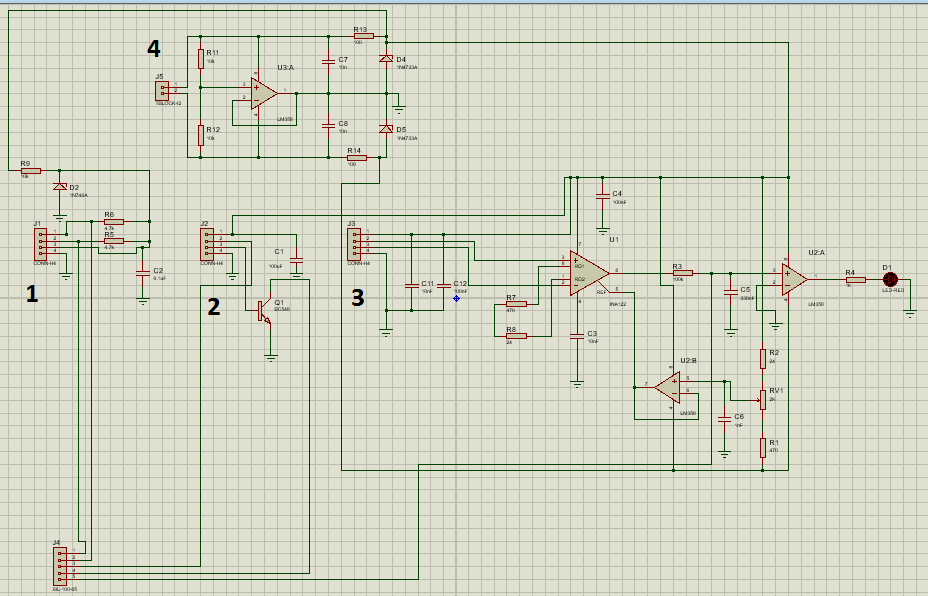
\includegraphics[scale=0.5]{esquematicosensores.png}
		\caption{Esquemático PCI de condicionamento dos sinais dos sensores}
		\label{esquemáticosensores}
	\end{figure}

	A Figura \ref{pcisensores} mostra a referida placa desenvolvida.

	\newpage
	\begin{figure}[!h]
		\centering
		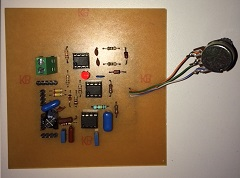
\includegraphics[scale=1]{pcisensores.png}
		\caption{Placa de Circuito Impresso de condicionamento dos sensores}
		\label{pcisensores}
	\end{figure}

	Nesse sentido, em termos de implementação de software, o sistema se baseia em acesso de threads responsáveis por controlar a rede de sensores e executar o controle. Acerca da rede de sensores, utilizando-se da API Xenomai foram implementadas tasks periódicas de um 1ms para cada sensor, logo a taxa de amostragem do sistema é fixa o que permite a comparação direta entre valores dos diferentes sensores. 

	Com o objetivo de contruir um sistema robusto foram implementadas diversas verificações de erro e funções específicas para gerenciar a execução do sistema, ou seja, foram definidas condições de contorno em caso de erro, como por exemplo, instâncias fantasmas.
	 
	\subsubsubsection{Módulo de Temperatura}

	Em função das características intrínsecas dos testes, optou-se por utilizar um sensor com medição sem contato, nesse caso o dispositivo faz uso de tecnologia baseada em sistema infravermelho para realizar a medição. Harmonizando os preceitos apresentados como requisitos do sistema e a questão levantada acima escolheu-se o sensor de temperatura Mlx90614, mostrado na Figura \ref{mlx}.

	\begin{figure}[!h]
		\centering
		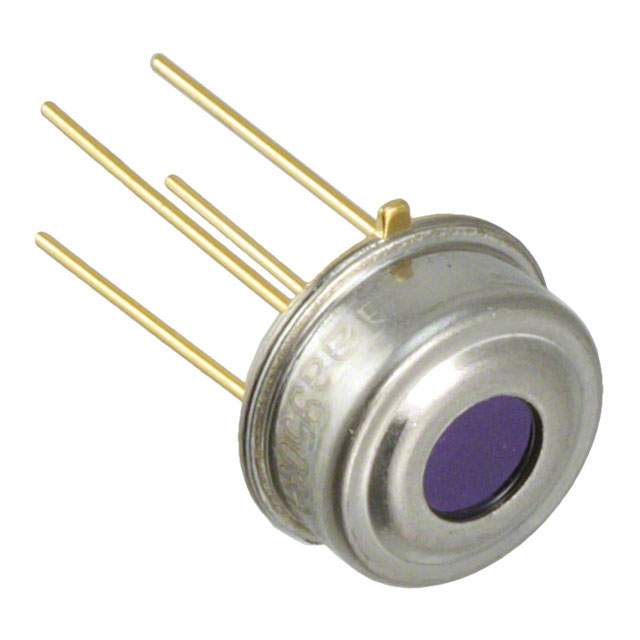
\includegraphics[scale=0.2]{mlx.png}
		\caption{Sensor MLX90614}
		\label{mlx}
	\end{figure}

	O MLX90614 possui uma máquina de estados interna que recebe e calcula a temperatura ambiente e do objeto. O MLX90614 possui a possibilidade de configurar o sinal de saída por PWM ou por interface I2C. No modo PWM o sensor possui uma resolução de $0.14^oC$ e no modo I2C uma resolução de $0.02^oC$, em virtude da melhor resolução optou-se pela utilização no modo I2C.

	Em termos de implementação, inicialmente deve-se configurar a comunicação entre o dispositivo master, a Beaglebone, e o dispositivo slave, o MLX90614. Segundo o protocolo, para realizar a leitura de dados inicialmente o dispositivo master deve enviar uma sequência de start e em seguida o endereço físico do dispositivo e o endereço de memória que deseja-se ler, envia-se novamente a sequência de start, solicita-se os dados de leitura e por fim envia-se a sequência de stop. 

	Os dados de leitura do senso, temperatura do objeto, são recebidos armazenados em um vetor de string em base hexadecimal, logo deve-se convertê-los para base decimal, e em seguida realizar a conversão de Kelvins para graus Celsius. 

	O bloco número 1 da Figura \ref{esquemáticosensores} corresponde a topologia sugerida pelo datasheet do MLX90614 para que o mesmo opere utilizando a interface I2C. Observa-se que o circuito trata-se de uma topologia com um capacitor de acoplamento e dois resistores de pullup, cujo objetivo é evitar flutuação de tensão nos pinos de entrada P9\_19 e P9\_20 da BeagleBone. A Tabela \ref{conexaotemperatura} apresenta a tabela de conexão do MLX90614.

	\begin{table}[!h]
	\centering
	\caption{Conexão para o MLX90614 J1}
	\vspace{0.5cm}
	\begin{tabular}{c c}
	\hline
	J1(1)			&	SCL P9\_19 BBB\\
	\hline
	J1(2)			&	SDA P9\_20 BBB\\
	\hline
	J1(3)			&	Vdd (3.3V)BBB\\
	\hline
	J1(4)			&	Gnd BBB\\
	\hline
	\label{conexaotemperatura}
	\end{tabular}
	\end{table}


	\subsubsubsection{Módulo de Sensoriamento de Velocidade}

	Em virtude da dificuldade de aferição da velocidade linear da haste optou-se pela utilização de um sensor de proximidade e implementar uma função de cálculo da taxa de variação da posição no tempo de amostragem. Em uma pesquisa de mercado optou-se pelo sensor HC-SR04 em virtude da sua fácil aquisição e faixa de operação larga. A Figura \ref{ultrassom} corresponde ao referido sensor e a Tabela \ref{descricaoHCSR04} aponta algumas de suas principais características.
	
	\begin{figure}[!h]
		\centering
		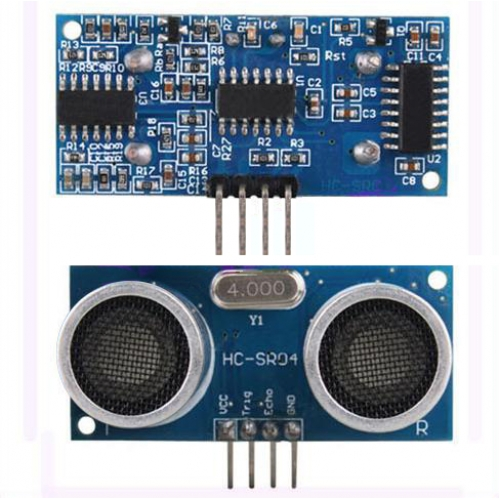
\includegraphics[scale=0.3]{ultrassom.png}
		\caption{Sensor HC-SR04}
		\label{ultrassom}
	\end{figure}

	\begin{table}[!h]
	\centering
	\caption{Características do Sensor HC-SR04}
	\vspace{0.5cm}
	\begin{tabular}{ c c}
	\hline
	\textbf{DESCRIÇÃO}	&	\textbf{VALOR}\\
	\hline
	Tensão de Alimentação DC & 5 V\\
	\hline
	Working Current & 15mA\\
	\hline
	Faixa de Operação & 2cm -  4m\\
	\hline
	Angulo de Medição &  $15^o$\\
	\hline
	Sinal de Trigger de entrada & $10\mu S$ TTL pulso\\
	\hline
	\label{descricaoHCSR04}
	\end{tabular}
	\end{table}

	\newpage
	O princípio de funcionamento do HC-SR04 pode ser entendido analisando-se o seu diagrama de tempo, como mostrado na figura \ref{diagramatempo}.

	\begin{figure}[!h]
		\centering
		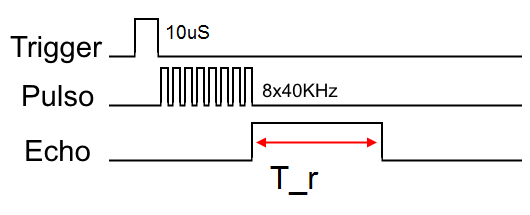
\includegraphics[scale=0.5]{diagrama_tempo_HCSR04.png}
		\caption{Diagrama de tempo do Sensor HC-SR04}
		\label{diagramatempo}
	\end{figure}

	Segundo o datasheet do HC-SR04, para iniciar a medição é necessário enviar um pulso de $10\mu S$ no pino de Trigger, o que corresponde a 8 pulsos de onda sonora visto que a frequência é de 40KHz, o pino de ECHO então fica em nível lógico alto até que seja detectado o sinal da onda refletida pelo objeto, de posse do tempo em que a entrada digital ECHO permanece em nível lógico alto é possível calcular a distância do objeto.

	O bloco 2 da Figura \ref{esquemáticosensores} corresponde a topologia empregada para o HC-SR04, como a BBB recebe um nível de tensão máximo de 3.3V nos seus pinos digitais é necessário adicionar uma topologia de proteção que garanta que o nível de tensão do ECHO do HC-SR04 seja menor que 3.3V. Optou-se pela utilização de um transistor NPN para realizar esse interfaceamento, assim como um capacitor de acoplamento. A Tabela \ref{conexaovelocidade} apresenta a tabela de conexão do HC-SR04.

	\begin{table}[!h]
	\centering
	\caption{Conexão para o HC-SR04 J2}
	\vspace{0.5cm}
	\begin{tabular}{c c}
	\hline
	J2(1)		&	Vdd 5V (FS)\\
	\hline
	J2(2)		&	Trigger P9\_25 BBB\\
	\hline
	J2(3)		&	Echo P9\_27 BBB\\
	\hline
	J2(4)		&	Gnd\\
	\hline
	\label{conexaovelocidade}
	\end{tabular}
	\end{table}

	\subsubsubsection{Módulo de Sensoriamento de Força}

	Segundo o escopo do projeto, a bancada será dimensionada para veículos leves. Comparando-se 3 modelos de veículos leves populares obteve-se os valores de massa máxima, como mostrado na Tabela \ref{comparativocarros}.

	\begin{table}[!h]
	\centering
	\caption{Comparativo de Veículos Leves e Populares}
	%\vspace{0.5cm}
	\begin{tabular}{ l c c c}
	\hline
	\textbf{VEÍCULO/MODELO} & \textbf{PESO BRUTO} & \textbf{PESO EM MARCHA}\\
	\hline
	NOVO UNO VIVACE 1.0 & 1295 Kg & 895 Kg\\
	\hline
	PÁLIO ATTRACTIVE 2014 & 1407 Kg & 1007 Kg\\
	\hline
	NOVO GOL 1.0 TOTAL FLEX & 1387 Kg & 947 Kg\\
	\hline
	\label{comparativocarros}
	\end{tabular}
	\end{table}

		A partir desses três modelos é possível obter um panorama geral para essa classe de veículos em termos de massa. Logo, observa-se que no pior dos casos,especificamente o pálio, dentro desse domínio é a massa de 351Kg em cada amortecedor. Portanto a bancada será projetada para no máximo 400Kg de carga, ou seja para amortecedores de veículos com peso bruto máximo de 1600kg. 
		
		Define-se o formato da célula de carga de acordo com a aplicação, como o carga é sustentada pela célula, é mais indicada a utilização de células em formato de S, por permitirem a aferição de força em movimentos de tração e compressão, além do fato de possuítem capacidade de trabalhar na faixa de valores necessária para o projeto.
		
		Em face dos aspectos apresentados, em uma pesquisa de mercado obteve-se o modelo a ser utilizado no presente projeto, como mostrado na Figura \ref{celuladecarga}.
	
	\newpage	
	\begin{figure}[!h]
		\centering
		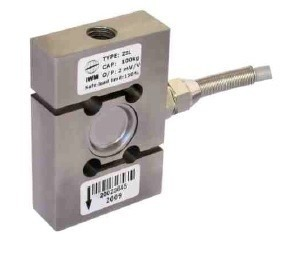
\includegraphics[scale=0.5]{celuladecarga.png}
		\caption{Célula de Carga - IWM ZSL 500Kg}
		\label{celuladecarga}
	\end{figure}

	Internamente a célula de carga possui uma ponte de Wheatstone responsável por reduzir os ruídos e aumentar a sensibilidade do sistema. Aplica-se uma tensão de referência de 5V e avalia-se a tensão entre os terminais Vs+ e Vs-, a aplicação de uma força implica em uma variação de resistência e consequentemente uma variação de tensão. A variação de tensão, no entanto, é muito baixa, a utilização de um amplificador de intrumentação torna-se necessária, pois o mesmo possui alto ganho e alta precisão, em seguida o sinal deve ser amplificado para um nível máximo de tensão de 1.8V,  que é a tensão máxima permitida nos pinos analógicos da BBB.

	Alimentando-se a célula com 5V, e sabendo que o dispositivo possui uma sensibilidade de 2,025mV/V e uma capacidade de 500Kg, conclui-se que a variação de 1Kg implica em uma variação de apenas $20,25\mu V$ por cada Kg. 

	 O terceiro bloco da Figura \ref{esquemáticosensores} corresponde a topologia empregada. Inicialmente utiliza-se capacitores com o objetivo de contribuir para a anulação do ripple de alta frequência, tornando a alimentação mais estável. Optou-se pela utilização de um INA126 para realizar a amplificação da diferença de potencial medida na célula de carga. 

	Como descrito no datasheet, o componente possui um balanço de zero de 0.0129mV o que significa que na ausência da aplicação de qualquer força a tensão observada será 0.0129, o que trata-se do erro sistemático de medição. Deve-se ajustar a tensão de referência do INA126, utilizou-se uma topologia de comparador de tensão em que é realizada uma comparação entre a saída Vout e a referência, ajusta-se então o potenciômetro, ligado à referência do INA126, até que o LED acenda, tal procedimento deve ser realizado sem carga para se obter a tensão Vout igual a zero para uma carga de 0Kg.

	A BBB possui 7 conversores AD de 12 bits,logo para a faixa de valores de tensão entre 0 e 1.8v obtém-se números discretos entre 0 e 4095. Segundo informações do datasheet do componente, a curva de sensibilidade pode ser descrita como uma reta com linearidade 0.02\%. Logo, para a faixa de operação do componente, existe uma relação linear entre a força aplicada e a tensão observada. A Tabela \ref{conexaoforca} apresenta a tabela de conexão 

	\begin{table}[!h]
	\centering
	\caption{Conexão para a célula de carga J3}
	\vspace{0.5cm}
	\begin{tabular}{c c}
	\hline
	J3(1)		&	Vdd 5V (FS)\\
	\hline
	J3(2)		&	IN+ INA16\\
	\hline
	J3(3)		&	IN- INA16\\
	\hline
	J3(4)		&	Gnd\\
	\hline
	LM358(P1)	&	P9\_39 BBB\\
	\hline
	\label{conexaoforca}
	\end{tabular}
	\end{table}

	\subsubsubsection{Fonte simétrica}

	O circuito de condicionamento da célula de carga utiliza fonte simétrica de $ \pm 5V $, nesse sentido implementou-se a topologia de fonte simétrica, referente ao bloco quatro, que utiliza-se do conceito de divisor de tensão, para dois resistores iguais, ou seja, as tensões entregues serão $\pm \frac{Vcc}{2}$ onde Vcc é a tensão fornecida. Para regular o nível de tensão em $\pm 5V$, utilizou-se diodos zener 1N4733, cuja tensão de ruptura é 5,1V.



	\subsubsection{PCI de interface com o inversor}

	O controle do teste se dará para três valores de velocidade fixas a serem selecionadas pelo usuário. Nesse sentido configurou-se o inversor de modo a fornecer três velocidades fixas selecionadas a partir da relação booleana entre duas entradas digitais. O nível de tensão, no entanto, das entradas digitais do inversor é de 24V e o nível de tensão de saída dos pinos digitais da Beaglebone é de 3.3V, logo foi necessária a implementação de um módulo de amplificação dos sinais provenientes da Beaglebone, como mostrado na Figura \ref{esquemáticoinversor}. 

	\begin{figure}[!h]
		\centering
		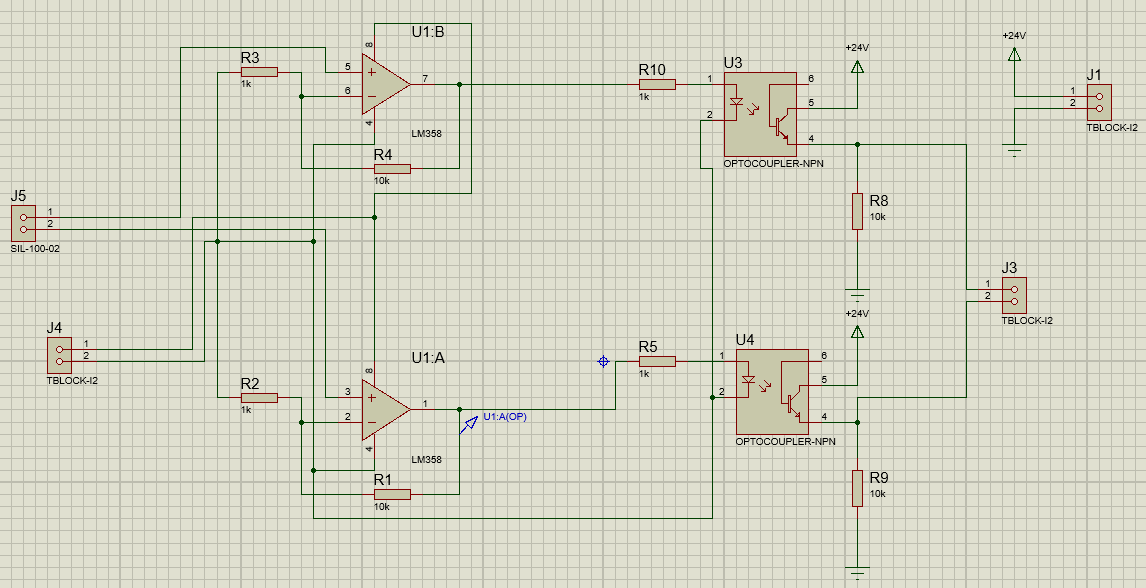
\includegraphics[scale=0.5]{esquematicoinversor.png}
		\caption{Esquemático PCI de interfaceamento com o inversor}
		\label{esquemáticoinversor}
	\end{figure}

	No intuito de proteger a Beaglebone contra possíveis surtos de corrente optou-se pela utilização de acopladores ópticos, que operam baseados no princípio de transmissão de sinais de um circuito para outro por meio de um feixe de luz, ou seja, sem contato físico, proporcionando portanto o isolamento total entre os pinos digitais da Beaglebone e o inversor.

	A Figura \ref{pciinversor} mostra a referida placa desenvolvida.
	\begin{figure}[!h]
		\centering
		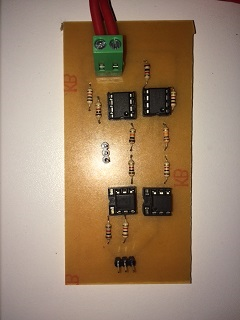
\includegraphics[scale=1]{pciinversor.png}
		\caption{Placa de de interfaceamento com o inversor}
		\label{pciinversor}
	\end{figure}

	Inicialmente implementou-se um módulo de amplificação cujo objetivo é amplificar o sinal proveniente da Beaglebone de 3.3V. Adotou-se a utilização da topologia não inversora, cujo ganho é expresso pela equação:
	$$ A = 1 + \frac{R2}{R1} $$
	Deseja-se obter uma tensão de 5V no pino 1 do opto-acoplador, logo os valores que satisfazem a equação acima são: $R2 = 10k\Omega$ e $ R1 = 2k\Omega $
	Optou-se por utilizar um resistor de $1k\Omega$ no ânodo do fotodiodo do opto-acoplador de modo a limitar a corrente que flui por ele dentro dos valores máximos do datasheet do componente, obtendo-se o valor de 5mA. Essa corrente é suficiente para acionar o fotodiodo que por sua vez excita o fototransistor, induzindo uma tensão de base, pois a mesma é sensível à luz. A tensão aplicada no coletor, 24V, então é induzida no emissor com uma queda de 0.5V, que corresponde à tensão de saturação do fototransistor.	
